\documentclass[tikz,border=8pt]{standalone}
% Shared look for every TikZ diagram. Load with \input{../../tools/tikz-style.tex}
\usepackage[T1]{fontenc}
\usepackage{lmodern}
\renewcommand{\sfdefault}{lmr}  % diagrams use the same serif as the text
\usetikzlibrary{arrows.meta, positioning, shapes.geometric, calc, fit, backgrounds}
\definecolor{cblue}{HTML}{4C78A8}
\definecolor{corange}{HTML}{F58518}
\definecolor{cgreen}{HTML}{54A24B}
\definecolor{cred}{HTML}{E45756}
\definecolor{cpurple}{HTML}{B279A2}
\definecolor{cgrey}{HTML}{6B6B6B}
\tikzset{
  every picture/.style={font=\sffamily, line width=1.2pt},
  box/.style={draw=#1, fill=#1!12, rounded corners=4pt, align=center, inner sep=7pt, minimum height=1.1cm},
  box/.default=cgrey,
  arrow/.style={-{Stealth[length=3mm]}, draw=cgrey, line width=1.4pt},
  title/.style={font=\sffamily\bfseries\Large},
  note/.style={font=\sffamily\small, text=cgrey, align=center},
}
\AtBeginDocument{\hyphenpenalty=10000 \exhyphenpenalty=10000}

\begin{document}
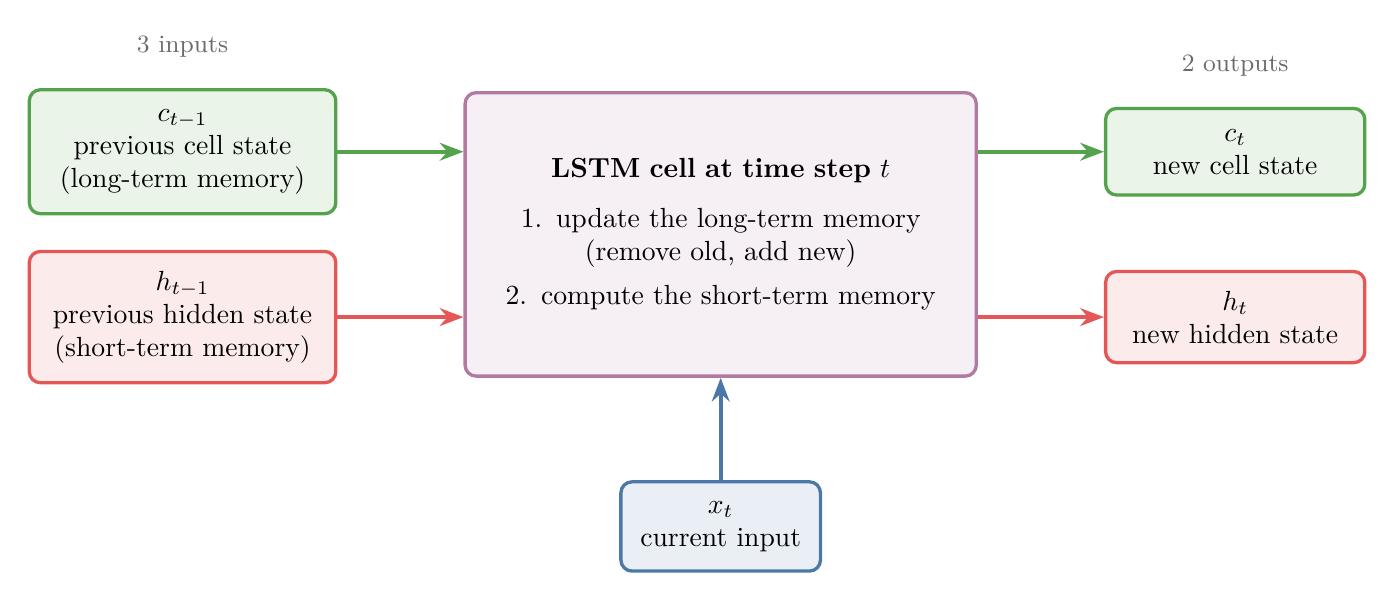
\begin{tikzpicture}
  \node[box=cpurple, minimum width=6.2cm, minimum height=3.6cm, text width=6cm] (cell)
    {\textbf{LSTM cell at time step $t$}\\[6pt]1. update the long-term memory\\(remove old, add new)\\[4pt]2. compute the short-term memory};
  \node[box=cgreen, text width=3.4cm, anchor=east] (cin) at ([xshift=-1.6cm, yshift=1.05cm]cell.west) {$c_{t-1}$\\previous cell state\\(long-term memory)};
  \node[box=cred, text width=3.4cm, anchor=east] (hin) at ([xshift=-1.6cm, yshift=-1.05cm]cell.west) {$h_{t-1}$\\previous hidden state\\(short-term memory)};
  \node[box=cblue, below=1.3cm of cell] (x) {$x_t$\\current input};
  \node[box=cgreen, text width=2.8cm, anchor=west] (cout) at ([xshift=1.6cm, yshift=1.05cm]cell.east) {$c_t$\\new cell state};
  \node[box=cred, text width=2.8cm, anchor=west] (hout) at ([xshift=1.6cm, yshift=-1.05cm]cell.east) {$h_t$\\new hidden state};
  \draw[arrow, draw=cgreen] (cin) -- (cin -| cell.west);
  \draw[arrow, draw=cred] (hin) -- (hin -| cell.west);
  \draw[arrow, draw=cblue] (x) -- (cell);
  \draw[arrow, draw=cgreen] (cout -| cell.east) -- (cout);
  \draw[arrow, draw=cred] (hout -| cell.east) -- (hout);
  \node[note, above=0.25cm of cin] {3 inputs};
  \node[note, above=0.25cm of cout] {2 outputs};
\end{tikzpicture}
\end{document}
